%%% ---------------
%%% PREAMBLE
%%% ---------------
\documentclass[10pt,a4paper]{article}

% Define geometry (without using the geometry package)
\usepackage{geometry}
\geometry{landscape, twocolumn, textwidth=27.0cm, textheight=19cm, columnsep=14mm}


\frenchspacing						% better looking spacing

% Call packages we'll need
\usepackage[french]{babel}			% french
\usepackage{graphicx}				% images
\usepackage{amssymb,amsmath}		% math
\usepackage{multicol}				% three-column layout
\usepackage{url}					% clickable links
\usepackage{marvosym}				% symbols
\usepackage{wrapfig}				% wrapping text around figures
\usepackage{fontspec}			% font encoding
\usepackage{xunicode}
\usepackage{ragged2e}
\usepackage{titlesec}
\usepackage{tocvsec2}
% Customize (header and) footer
\usepackage{fancyhdr}
\usepackage{enumitem}
%\pagestyle{fancy}
\pagestyle{empty}

%\titlespacing\section{0pt}{0pt plus 4pt minus 2pt}{0pt plus 2pt minus 2pt}
%\titlespacing\subsection{0pt}{12pt plus 4pt minus 2pt}{0pt plus 2pt minus 2pt}
%\titlespacing\subsubsection{0pt}{12pt plus 4pt minus 2pt}{0pt plus 2pt minus 2pt}

%\newfontfamily\headingfont[]{Arial}
%\titleformat*{\section}{\Large\bfseries\sffamily}
%\titleformat*{\section}{\Large\headingfont}

%\renewcommand{\headrulewidth}{0.0pt}	% no bar on top of page
%\renewcommand{\footrulewidth}{0.4pt}	% bar on bottom of page

%%% ---------------
%%% DEFINITIONS
%%% ---------------

% Define separators
\newcommand{\HorRule}[1]{\noindent\rule{\linewidth}{#1}} % Creating a horizontal rule
\newcommand{\SepRule}{\noindent							 % Creating a separator
						\begin{center}
							\rule{250pt}{1pt}
						\end{center}
						}						

% Define Title en News input
\newcommand{\JournalName}[1]{%
		\begin{center}	
			%\Huge \usefont{T1}{augie}{m}{n}
            \Large \usefont{T1}{augie}{m}{n}
			#1%
		\end{center}	
		\par \normalsize \normalfont}
		
\newcommand{\JournalIssue}[1]{%
		\hfill \textsc{\mydate \today, No #1}
		\par \normalsize \normalfont}

\newcommand{\NewsItem}[1]{%
\vspace{4pt}
		%\usefont{T1}{augie}{m}{n} 	
		\large \textbf{#1} \vspace{4pt}
        %\Large #1 \vspace{4pt}
		%\par 
        \normalsize \normalfont}
		
\newcommand{\NewsAuthor}[1]{%
			\hfill by \textsc{#1} \vspace{4pt}
			\par \normalfont}		

%pas de numérotation des sections
\setsecnumdepth{none}
%%% ---------------
%%% BEGIN DOCUMENT
%%% ---------------
\begin{document}
% Title	
% -----




% Other news (1)
% -----
%\vspace{0.5cm}
%	\SepRule
%\vspace{0.5cm}

\textit{Rassemblement à la grotte pour la bénédiction des rameaux}
\NewsItem{Bénédiction des rameaux}
	Par la croix du Serviteur, porche royal où s'avancent les pécheurs\\
Par le corps de Jésus Christ, nu, outragé sous le rire des bourreaux\\
Sur les foules sans berger et sans espoir qui ne vont qu'à perdre cœur\\
Fais paraitre ton jour et le temps de ta grâce, fais paraitre ton jour, que l’homme soit sauvé

\NewsItem{Évangile} Luc 19,28-40
\NewsItem{Entrée en procession}

	\NewsItem{Chant d'entrée}
	%\section{Chant d'entrée}
	\begin{itemize}
\item[R/] Hosanna, Hosanna, Hosanna au plus haut des cieux !
\item[]
Saint, saint, saint, le Seigneur, Dieu de l'univers.
\item[]
Le ciel et la terre sont remplis de ta gloire. R/
\item[]
Béni soit celui qui vient au nom du Seigneur. R/
\end{itemize}

\NewsItem{Chant d'entrée}

% -----
%\section{Préparation pénitentielle}
\NewsItem{Préparation pénitentielle}
Seigneur, prends pitié. Seigneur prends pitié, Seigneur, prends pitié\\
Ô Christ, prends pitié. ô Christ prends pitié, o Christ, prends pitié.\\
Seigneur, prends pitié. Seigneur, prends pitié Seigneur, prends pitié

% -----

\NewsItem{Gloire à Dieu}  
\begin{itemize}
\item[R/] 
Gloire à Dieu, au plus haut des cieux, et paix sur la terre, aux hommes qu'il aime. (bis)
\item[1.]
Nous te louons, nous te bénissons, nous t’adorons, nous te glorifions, nous   
      te rendons grâce pour ton immense gloire. Seigneur Dieu, Roi du ciel, Dieu 
      le Père tout puissant. R/
\item[2.]
Jésus-Christ, Seigneur Fils unique, Agneau de Dieu, le Fils du Père, toi qui 
      enlèves le péché du monde, reçois nos prières. Toi qui es assis à la droite  
      du Père, prends pitié de nous. R/
\item[3.]
Car toi seul es saint, toi seul es Seigneur, toi seul es le Très Haut : 
      Jésus-Christ, avec le Saint Esprit, dans la gloire de Dieu le Père. R/
\end{itemize}



% -----
\NewsItem{Première lecture}
\og Me voici : envoie-moi ! \fg (Is 6, 1-2a.3-8)
% -----

\NewsItem{Psaume}
Ps 18A (19), 2-3, 4-5ab

\textbf{Le jour où je t’appelle, réponds-moi, Seigneur.}

\smallskip

De tout mon cœur, Seigneur, je te rends grâce :
tu as entendu les paroles de ma bouche.
Je te chante en présence des anges,
vers ton temple sacré, je me prosterne.

\smallskip

Je rends grâce à ton nom pour ton amour et ta vérité,
car tu élèves, au-dessus de tout, ton nom et ta parole.
Le jour où tu répondis à mon appel,
tu fis grandir en mon âme la force.

\smallskip

Si haut que soit le Seigneur, il voit le plus humble ;
de loin, il reconnaît l’orgueilleux.
Si je marche au milieu des angoisses, tu me fais vivre,
ta main s’abat sur mes ennemis en colère.

\smallskip

Ta droite me rend vainqueur.
Le Seigneur fait tout pour moi !
Seigneur, éternel est ton amour :
n’arrête pas l’œuvre de tes mains.


% -----
\NewsItem{Deuxième lecture}
\og Voilà ce que nous proclamons, voilà ce que vous croyez \fg (1 Co 15, 1-11)

% -----

\NewsItem{Acclamation} : Alléluia, Alléluia ! (4 fois)
% -----

% -----
\NewsItem{Évangile} : \og Laissant tout, ils le suivirent \fg (Lc 5, 1-11)
% -----


\NewsItem{Profession de foi} 


\NewsItem{Prières universelles} 
Entends Seigneur la prière, qui monte de nos cœurs.
\newpage

\NewsItem{Offertoire} 
Venez à moi, vous qui portez un fardeau 
\begin{itemize}
\item[R/] Venez à moi, vous qui portez un fardeau. Venez, vous tous qui peinez. 
     Et moi, je vous soulagerai. Je suis le repos de vos âmes.
\item[1.]  Mettez-vous à mon école, car je suis doux, je suis humble de cœur. Prenez 
      mon joug, il est aisé et vous trouverez la paix. Mon fardeau est léger !
\item[2.]
Devant toi je tiens mon âme, comme un enfant dans les bras de sa mère. Seigneur, mon âme espère en toi ! En silence et dans la foi, j'espère le Seigneur !
\end{itemize}

\NewsItem{Prières sur les offrandes}
\textit{Nous nous levons et nous répondons : }

Que le Seigneur reçoive de vos mains ce sacrifice à la louange et à la gloire 
de Son nom, pour notre bien et celui de toute l’Église.

\NewsItem{Sanctus}
\begin{itemize}
\item[R/] Trois fois Saint, trois fois Saint, le Seigneur Dieu de l’univers. 
      Hosanna, hosanna (bis) au plus haut des Cieux ! 
\item[1.]  Le Ciel et la Terre nous chantent Ta gloire, hosanna au plus haut des Cieux. 
      Béni soit Celui qui vient, c’est Jésus notre Sauveur ! 
\end{itemize}

\NewsItem{Anamnèse}
Gloire à Toi qui étais mort. Gloire à Toi qui est vivant.  
Notre Sauveur et notre Dieu, viens, Seigneur Jésus.

\NewsItem{Notre Père}

\NewsItem{Geste de paix}
Donne la paix, Seigneur, donne Ta paix ! (bis) 

\NewsItem{Agnus}
\begin{itemize}
    \item 
    Agneau de Dieu qui enlèves les péchés du monde, prends pitié de nous (bis)
    \item
Agneau de Dieu qui enlèves les péchés du monde, donne-nous la paix
\end{itemize}

\NewsItem{Communion} Pour former un seul corps
\begin{itemize}
    \item [1.]
    Pour former un seul corps, boire à la même coupe, pour former un
       seul corps, comme des milliers de grains ne font qu’un bout de pain. 
       Pour former un seul corps, boire à la même coupe, pour former un seul 
       corps et que l’on soit d’accord pour que règne l’amour…
\item[R/]  Mangeons ce pain, le pain vivant, buvons ce vin qui est son sang, corps               
       et sang de Jésus-Christ, pour suivre son chemin et devenir témoins.

\item[2.]    Pour former un seul corps, boire à la même coupe, pour former un 
        seul corps, comme des milliers de grains n’offrent qu’un peu de vin. 
        Pour former un seul corps, boire à la même coupe, pour former un seul 
        corps, donner chacun de soi pour que règne la joie…
\end{itemize}

\newpage

\NewsItem{Envoi} Allons dire partout comment Jésus est bon
\begin{itemize}
    \item [R/] Allons dire partout comment Jésus est bon (bis) oui chantons partout, ne gardons 
     pas ça pour nous, allons chanter partout les merveilles qu’il fait pour nous !
\item[1.]  Il me fait découvrir comme la vie en Lui est jolie, quand je marche avec Lui, quand je marche 
     avec Lui. Il me fait retrouver la confiance que j’avais perdue, me rend tellement content,  
     que je chante son nom tout le temps !
\item[3.] Il me fait découvrir comment l’amour en Lui fleurit, quand je suis son chemin, quand je suis 
     son chemin. Il me fait retrouver toute la joie que j’avais perdue, me rend tellement content,  
     que je chante son nom tout le temps !
     \end{itemize}

     \NewsItem{Informations paroissiales}
             
         \begin{tabular}{l l l}
         \multicolumn{3}{c}{\textbf{St Jean-Baptiste}} \\
  Mardi & 11 fév. & Vêpres 18h15 - 18h30. Pas de messe \\
Jeudi & 13 fév. & Salut au Saint Sacrement 18h15. Messe 18h30. \\
    Vendredi & 14 fév. & Laudes 08h45 - 09h00. Pas de messe \\
        Samedi  & 15 fév. & Messe anticipée 18h00 \\
    Dimanche & 16 fév. & Pas de messe \\      
      
         \multicolumn{3}{c}{\textbf{Ste Croix}} \\
         Mercredi & 12 fév. & Pas de messe \\ 
         Dimanche & 16 fév.& Messe 10h30 \\
    
        \end{tabular}
  

\newpage

\JournalName{Communauté de Paroisses de Lingolsheim \\
\normalsize \textit{Notre Dame des Sables}
\\ \large \'{E}glise Saint Jean-Baptiste
\\  \normalsize \textit{5ème dimanche du Temps Ordinaire - année C}
\\ \large Samedi 08 février 2025 à 18h00}
%\noindent\HorRule{3pt} \\[-0.75\baselineskip]
%\HorRule{1pt}
% -----

% Front article
% -----
%\vspace{0.5cm}
%	\SepRule
%\vspace{0.5cm}

%\begin{center}
\begin{minipage}[h]{1.0\linewidth}
 \begin{center}
 \textbf{
 %\dots
\og 
Rentrée Pastorale 2025-2026
 \fg{}
 %\dots
 }
 \end{center}

%\begin{wrapfigure}{l}{1.3cm}
%\vspace{-0.4cm}
%	\includegraphics[scale=1.0]{../images/lazarre}
%\end{wrapfigure}
Une nouvelle rentrée pastorale qui nous réjouit tous. En effet, après un temps de répit, il nous revient de mettre en marche la machine de nos activités pastorales.

Au début de cette nouvelle année pastorale, je souhaite vous redire toute ma joie de vous retrouver pour continuer la mission qui m’est assignée dans notre communauté de paroisses. Et comme chaque année, nous mettrons l’accent en premier lieu sur la vie catéchétique des enfants et des adolescences, l’animation liturgique, la création d’une troisième chorale, la visite aux malades et dans notre maison de retraite ( \emph{Résidence du Parc}), l’accueil et l’accompagnement en vue de baptêmes,  du catéchuménat des adultes, des mariages, l’encadrement  des servants d’autel, l’entretien de notre église pour la rendre  accueillante, avec ces innombrables petits gestes de service qui jalonnent l’existence ; tout cela nous aidera à vivre une véritable dimension ecclésiale.

Je voudrais vous remercier de tout cœur, vous tous qui êtes des membres vivants et actifs de la communauté paroissiale que nous formons, véritable artisans de l’évangélisation ordinaire. Mon souhait pour la vie de notre communauté de paroisses est que nous arrivions toujours plus à nous ouvrir et à nous connaître les uns les autres, à nous apprécier dans ce que nous sommes et vivons.

L’année dernière, avec toutes les entités de nos deux paroisses, nous avons eu différentes propositions, activités et invitations qui ont favorisées l’\textbf{Unité et l’ouverture} qui constituaient notre thème pastoral. Ne manquons pas cette année ces moments simples et conviviaux qui permettent de tisser des liens gratuits, profonds et tout simplement chrétiens.

\begin{wrapfigure}{l}{1.2cm}
\vspace{-0.4cm}
	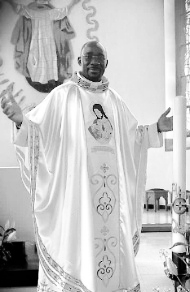
\includegraphics[scale=1.20]{../images/standing_daniel}
\end{wrapfigure}
Cette année nous porterons ensemble cette rentrée dans le cœur de chacun avec nos \textbf{jeunes pro}. Chacun à son rythme, selon ses possibilités et ses réalités mais avec un seul et même objectif : l’accomplissement de nos activités communautaires. Présentons également notre rentrée paroissiale au Christ. Et continuons notre chemin pour la mise en œuvre de notre projet paroissial autour de ce principal thème : \textbf{\og Avec notre jeunesse bâtissons une communauté plus dynamique, rayonnante et missionnaire\fg{}.}

	Que cette rentrée pastorale nous aide à prendre des résolutions nécessairement pour plonger à frais nouveaux dans la parole et être des disciples crédibles de l’évangile.


\begin{flushright}
Bonne rentrée pastorale à toutes et à tous !
\textit{Père  Daniel  ETTÉ}
\end{flushright}


\end{minipage}
%\end{center}
% -----


% Other news (2)
% -----
%\section{Elephant eats frog}
%\NewsAuthor{J. Doe}
%	\blindtext[1]
%		\begin{center}
%			\includegraphics[width=0.8\linewidth]{elephant}
%		\end{center}
%		\blindtext[1]

% -----
\end{document} 
